% !TEX root = thesis.tex
\documentclass[12pt,a4paper,titlepage,listof=totoc,bibliography=totoc,chapteratlists=0pt]{scrreprt}
\usepackage{amsfonts, amssymb, amsmath, verbatim, float}
\usepackage{listings}

\lstdefinestyle{yaml}{
     basicstyle=\color{blue}\footnotesize,
     rulecolor=\color{black},
     string=[s]{'}{'},
     stringstyle=\color{blue},
     comment=[l]{:}, 
     commentstyle=\color{black},
     morecomment=[l]{-}
 }

 \lstdefinelanguage{JavaScript}{
  morekeywords=[1]{break, continue, delete, else, for, function, if, in,
    new, return, this, typeof, var, void, while, with},
  % Literals, primitive types, and reference types.
  morekeywords=[2]{false, null, true, boolean, number, undefined,
    Array, Boolean, Date, Math, Number, String, Object},
  % Built-ins.
  morekeywords=[3]{eval, parseInt, parseFloat, escape, unescape},
  sensitive,
  morecomment=[s]{/*}{*/},
  morecomment=[l]//,
  morecomment=[s]{/**}{*/}, % JavaDoc style comments
  morestring=[b]',
  morestring=[b]"
}[keywords, comments, strings]
\begin{filecontents*}{\jobname.xmpdata}
	\Keywords{CHANGEME, VR, IOT, TODO}
	\Title{CHANGEME: Unser tolles Thema -- wir sind suppa}
	\Author{CHANGEME, Stefan Schwammal, Susi Schwammal}
\end{filecontents*}

\setcounter{tocdepth}{1}

\usepackage[utf8]{inputenc}
\usepackage[T1]{fontenc}
\usepackage{amsmath}
\usepackage{amsfonts}
\usepackage{amssymb}
\usepackage[table]{xcolor}
\usepackage{graphicx}
\usepackage[left=3.50cm, right=2.00cm, top=2.00cm, bottom=2.00cm,foot=1cm]{geometry}
\usepackage[splitrule,hang,flushmargin,multiple,bottom]{footmisc}
\usepackage{lmodern, textcomp}
\usepackage{lmodern}
\usepackage{pdfpages}
\usepackage[ngerman]{babel}
\usepackage{multicol}
\usepackage{float}
\usepackage{array,tabularx,booktabs}
\usepackage{ragged2e}
\usepackage{lipsum}
\usepackage{wrapfig}

\newcolumntype{M}[1]{>{\centering\arraybackslash}m{#1}}

\usepackage{enumitem}
\newlist{compactitem}{itemize}{3}
\setlist[compactitem,1]{label=\textbullet, nosep,leftmargin=1.5em,labelwidth=*,align=left}
\setlist[compactitem,2]{label=--, nosep,leftmargin=1.5em,labelwidth=*,align=left}
\setlist[compactitem,3]{label=\textopenbullet, nosep,leftmargin=1.5em,labelwidth=*,align=left}
\newlist{compactenum}{enumerate}{3}
\setlist[compactenum,1]{label=\arabic*., nosep,leftmargin=1.5em,labelwidth=*,align=left}
\setlist[compactenum,2]{label=\alph*., nosep,leftmargin=1.5em,labelwidth=*,align=left}
\setlist[compactenum,3]{label=\roman*., nosep,leftmargin=1.5em,labelwidth=*,align=left}
\newlist{compactdesc}{description}{3}
\setlist[compactdesc]{leftmargin=1.5em,labelwidth=*,align=left}

\usepackage{microtype}

\usepackage[parfill]{parskip}

\definecolor{bluekeywords}{rgb}{0.13,0.13,1}
\definecolor{greencomments}{rgb}{0,0.5,0}
\definecolor{redstrings}{rgb}{0.9,0,0}
\definecolor{lightgray}{gray}{0.9}
\definecolor{lightblue}{rgb}{0.93,0.95,1.0}

\usepackage{listings}

\makeatletter
\lstdefinestyle{lststyle}{
	basicstyle=%
	\ttfamily
	\lst@ifdisplaystyle\scriptsize\fi
}
\makeatother

\renewcommand{\lstlistlistingname}{List of Listings}
% TODO: define other languages as needed
\lstset{language=Python,
numbers=left,               
numberstyle=\tiny,          
showspaces=false,
showtabs=false,
breaklines=true,
lineskip=-1pt,
tabsize=2,
showstringspaces=false,
breakatwhitespace=true,
escapeinside={(*@}{@*)},
commentstyle=\color{greencomments},
keywordstyle=\color{bluekeywords}\bfseries,
stringstyle=\color{redstrings},
style=lststyle,
xleftmargin=17pt,
         framexleftmargin=17pt,
         framexrightmargin=5pt,
         framexbottommargin=4pt
}
\lstset{
morekeywords={base,var,in,out,dynamic,from,where,select,orderby,function,\$,group,by,into,yield,async,await,@,None,self,as,elif,with}
}
\lstdefinelanguage{TypeScript}{
	keywords={typeof, new, true, false, catch, function, return, null, switch, var, if, in, while, do, else, case, break, void, number, string, boolean, module, \$, export, for, this},
	keywordstyle=\color{blue}\bfseries,
	ndkeywords={class, export, boolean, throw, implements, import, this},
	ndkeywordstyle=\color{darkgray}\bfseries,
	identifierstyle=\color{black},
	sensitive=false,
	comment=[l]{//},
	morecomment=[s]{/*}{*/},
	commentstyle=\color{purple}\ttfamily,
	stringstyle=\color{red}\ttfamily,
	morestring=[b]',
	morestring=[b]"
}
\usepackage{caption}
\DeclareCaptionFont{white}{\color{white}}
\DeclareCaptionFormat{listing}{\colorbox[cmyk]{0.43, 0.35, 0.35,0.01}{\parbox{\textwidth}{\hspace{10pt}#1#2#3}}}
\captionsetup[lstlisting]{format=listing,labelfont=white,textfont=white} 
\captionsetup[table]{justification=centering, singlelinecheck=false}

\usepackage{subcaption}

\usepackage{setspace}
\newcommand{\MSonehalfspacing}{%
	\setstretch{1.44}%  default
	\ifcase \@ptsize \relax % 10pt
	\setstretch {1.448}%
	\or % 11pt
	\setstretch {1.399}%
	\or % 12pt
	\setstretch {1.433}%
	\fi
}

\newcommand{\setauthor}[1]{\ohead[]{#1}}

\usepackage[automark]{scrlayer-scrpage}
\pagestyle{scrheadings}
\automark{chapter}
\renewcommand\sectionmark[1]{\markright{\MakeMarkcase {\thesection\hskip .5em\relax#1}}}
\rohead{\ifnum\expandafter\pdfstrcmp\botmark=0 \rightmark\else\leftmark{} --- \rightmark\fi}
\ihead[]{\headmark}
\chead[]{}
\ohead{}
\cfoot[]{}
\ofoot[\pagemark]{\pagemark}
\setheadsepline{.1pt}

\usepackage[hyphens]{url}

\usepackage[a-1b]{pdfx}

\usepackage{hyperref}
\hypersetup{pdfa}

\usepackage[nonumberlist,toc,nopostdot]{glossaries}

\usepackage{chngcntr}
\counterwithout{footnote}{chapter}
\counterwithout{figure}{chapter}
\counterwithout{table}{chapter}
\AtBeginDocument{
	\counterwithout{lstlisting}{chapter}
	\urlstyle{sf}
}
\newcounter{RPages}

\makeatletter
\def\bstctlcite{\@ifnextchar[{\@bstctlcite}{\@bstctlcite[@auxout]}}
\def\@bstctlcite[#1]#2{\@bsphack
	\@for\@citeb:=#2\do{%
		\edef\@citeb{\expandafter\@firstofone\@citeb}%
		\if@filesw\immediate\write\csname #1\endcsname{\string\citation{\@citeb}}\fi}%
	\@esphack}
\makeatother

\clubpenalty=10000 
\widowpenalty=10000
\displaywidowpenalty=10000
\interfootnotelinepenalty=10000

\title{Dynamische Anpassung von .Net Anwendungen zur Laufzeit}
\author{Robert Freiseisen, Philipp Füreder}

\makeindex
\makeglossaries
\begin{document}
\bstctlcite{IEEEexample:BSTcontrol}
\newcommand{\reminder}[1]
{ \textcolor{red}{<[{\bf\marginpar{\mbox{$<==$}} #1 }]>} }
\newcommand{\icode}[1]{\lstinline$#1$}
%\urlstyle{same}
%\setstretch{1.5}
\setstretch {1.433}
\renewcommand{\arraystretch}{1.2}


\includepdf{./titlepage/coversheet.pdf}
\pagenumbering{Roman}
\newpage
\thispagestyle{empty}
\vspace{3cm}
~ \\ \\
Ich erkläre an Eides statt, dass ich die vorliegende Diplomarbeit selbstständig und ohne fremde Hilfe verfasst, andere als die angegebenen Quellen und Hilfsmittel nicht benutzt bzw. die wörtlich oder sinngemäß entnommenen Stellen als solche kenntlich gemacht habe.

Die Arbeit wurde bisher in gleicher oder ähnlicher Weise keiner anderen Prüfungsbehörde vorgelegt und auch noch nicht veröffentlicht.

Die vorliegende Diplomarbeit ist mit dem elektronisch übermittelten Textdokument identisch.
\vspace{3cm}
% Hier kommt die Unterschrift drüber
\begin{tabbing}
Leonding, Dezember 2023 \hspace{5cm} P. Füreder \& R. Freiseisen
\end{tabbing}
\vspace{10cm}
\newpage
\setcounter{page}{1}

\begin{spacing}{1}
    \chapter*{Abstract}
\end{spacing}
\begin{wrapfigure}{r}{0.3\textwidth}
    \begin{center}
      
\includegraphics[width=0.2\textwidth]{pics/question_mark.png}
    \end{center}
\end{wrapfigure}
Brief summary of our amazing work. In English.
This is the only time we have to include a picture within the text.
The picture should somehow represent your thesis.
This is untypical for scientific work but required by the powers that are.
\lipsum[6]
\newpage
\begin{spacing}{1}
    \chapter*{Zusammenfassung}
\end{spacing}
\begin{wrapfigure}{r}{0.3\textwidth}
    \begin{center}
      
\includegraphics[width=0.2\textwidth]{pics/question_mark.png}
    \end{center}
\end{wrapfigure}
Zusammenfassung unserer genialen Arbeit. Auf Deutsch.
Das ist das einzige Mal, dass eine Grafik in den Textfluss eingebunden wird.
Die gewählte Grafik soll irgendwie eure Arbeit repräsentieren.
Das ist ungewöhnlich für eine wissenschaftliche Arbeit aber eine Anforderung der Obrigkeit.
\emph{Bitte auf keinen Fall mit der Zusammenfassung verwechseln, die den Abschluss der Arbeit bildet!}
\lipsum[6]


\pagestyle{plain}

\renewcommand{\lstlistlistingname}{Quellcodeverzeichnis}

\tableofcontents
\newpage
\setcounter{RPages}{\value{page}}
\setcounter{page}{0}
\pagenumbering{arabic}
\pagestyle{scrheadings}

\begin{spacing}{1}
\chapter{Einleitung}\label{chapter:introduction}
\end{spacing}
\section {Standardsoftware vs Individualsoftware}
\setauthor{Philipp Füreder}

In der heutigen digitalisierten Welt ist Software enorm wichtig für den Erfolg von Unternehmen 
oder auch für den privaten Gebrauch.
Es gibt zwei Hauptarten von Software, die von Unternehmen genutzt werden: \textbf{Standardsoftware} und 
\textbf{Individualsoftware}.
Beide haben Vor- und Nachteile, und es ist wichtig, 
diese gut zu verstehen, um die richtige Wahl für das eigene Unternehmen zu treffen.

\subsection*{Standardsoftware}

Standardsoftware ist üblicherweise sehr Benutzerfreundlich und einfach zu verwenden. 
Sie wird meist von großen Unternehmen entwickelt 
(Beispiel: Microsoft Office, Adobe Creative Cloud oder auch Google Workspace) 
und ist in der Anschaffung billiger als Individualsoftware. 
Der Grund dafür ist, dass Standardsoftware für die breite Masse entwickelt wird 
und für jeden Nutzer die gleichen Funktionen besitzt. 
Außerdem sind sie in der Regel weiter verbreitet und leichter zu erwerben.

Ein Nachteil von Standardsoftware besteht darin, dass sie nicht immer genau 
den individuellen Anforderungen eines Unternehmens gerecht wird. 
Es könnte vorkommen, dass spezifische Funktionen fehlen oder die Software 
nicht optimal auf die Arbeitsprozesse des Unternehmens zugeschnitten ist. 
\newpage
\subsection*{Individualsoftware}

Auf der anderen Seite wird Individualsoftware speziell für ein einzelnes 
Unternehmen oder eine bestimmte Aufgabe entworfen. 
Das bedeutet, es ist eine individuelle Lösung, die exakt auf 
die Anforderungen und Bedürfnisse der Benutzer/innen zugeschnitten ist.

Die Verwendung von Individualsoftware hat aber auch ihre Nachteile. 
Zum einen ist sie in der Regel kostenintensiver, da die individuelle Entwicklung 
mehr Ressourcen erfordert. Zum anderen gestaltet sich die Umsetzung und Wartung 
anspruchsvoller, da die Einzigartigkeit der Software spezifische Herausforderungen 
mit sich bringt, die über die Zeit hinweg bewältigt werden müssen.

\section{Problemverständnis}

Die meisten Benutzer/innen sind mit den gängigsten Standardsoftwares bereits vertraut. 
Deshalb wäre eine neue Individualsoftware eine Umstellung, wo man wieder Zeit aufwenden muss, 
um sich damit zurecht zu finden. Und außerdem muss man diese dann ja auch implementieren (als Entwickler), 
warten und vor allem finanzieren, was sehr kostspielig sein kann. 
\newline
Es mag verlockend sein, Standardsoftware mit den benötigten Funktionen für jeden Kunden anzupassen. 
Aber das bringt viele Probleme mit sich. Wenn man für jeden Kunden 
spezielle Funktionen einbaut, muss man den Software-Code jedes Mal stark ändern. 
Das macht die Software kompliziert und schwer zu pflegen. Es können auch Fehler auftreten, 
wenn neue Funktionen hinzugefügt werden, und es wird schwierig, die Software auf dem 
neuesten Stand zu halten.

\newpage
\section{Lösungsansatz: Scripting}
\setauthor{Philipp Füreder}

Ein vielversprechender Ansatz zur Lösung von fehlenden Funktionen in einer Software besteht darin 
Scripting zu nutzen. Dadurch erhalten Benutzer/innen die Möglichkeit, eigene Scripts zu erstellen, 
um spezifische Funktionen innerhalb der Software auszuführen. Diese Scripts werden 
zur Laufzeit in die Anwendung geladen.

\subsection*{Allgemeines zu Scripting}

Scripting ermöglicht es individuelle Lösungen zu erstellen, 
die den eigenen Anforderungen gerecht werden. 
Dies erweitert den Nutzen der Software, ohne auf offizielle Updates oder neue Versionen 
warten zu müssen oder sogar eine eigene Software entwickeln zu müssen.

Eine Skriptsprache wird vor allem verwendet, um Websites und Webanwendungen zu automatisieren. 
Wenn man ein Skript schreibt, baut man kein völlig neues Programm von Grund auf. 
Stattdessen verknüpft man bestehende Teile eines Programms miteinander. 
Dann führt das Programm dieses Skript aus.

Ein zentraler Aspekt dieser Diplomarbeit war die Untersuchung der Rolle des Scripting 
bei der dynamischen Anpassung von .NET-Anwendungen. Der Einsatz von Skriptsprachen ermöglicht es, 
fehlende oder zusätzliche Funktionen zur Laufzeit in eine Anwendung zu integrieren. 
Im Rahmen unserer Arbeit wurde verschiedenen Skriptsprachen experimentiert, um deren 
Eignung für die Integration in .NET-Anwendungen zu bewerten. Insbesondere wurde erforscht, 
wie Skripte nahtlos in die .NET-Anwendungen eingebettet und ausgeführt werden können, um die 
Flexibilität und Erweiterbarkeit der Anwendungen zu erhöhen. 

\newpage

\subsection*{Vorteile}

\begin{itemize}
    \item \textbf{Schnelle Entwicklung:} Skriptsprachen werden interpretiert, 
    wodurch Code rasch entwickelt und getestet werden kann. 
    Dies ermöglicht ein einfaches Ausprobieren neuer Ideen und die zügige 
    Erzielung von Ergebnissen, was Skriptsprachen besonders für interaktive 
    Programmieransätze geeignet macht.
    \item \textbf{Benutzerfreundlichkeit:} Skriptsprachen zeichnen sich durch ihre 
    Benutzerfreundlichkeit aus, wobei der Fokus auf der simplen und intuitiven 
    Gestaltung gängiger Aufgaben liegt. Diese Eigenschaft eignet sich perfekt für Anfänger 
    sowie für Aufgaben, die keine umfangreiche Rechenleistung erfordern.
    \item \textbf{Flexibles Verhalten:} Häufig weisen Skriptsprachen eine dynamische 
    Typisierung auf, die es ermöglicht, dass der Typ einer Variablen während der 
    Laufzeit verändert werden kann. Dies vereinfacht die Erstellung flexiblen und 
    anpassungsfähigen Codes sowie den Umgang mit Daten in vielfältigen Formaten.

\end{itemize}

\subsection*{Nachteile}

\begin{itemize}
    \item Der größte Nachteil von Skriptsprachen ist, dass sie langsamer sind als 
    andere Programmiersprachen. Das liegt daran, dass in Skriptsprachen jedes 
    Statement nacheinander während der Ausführung gelesen und verarbeitet wird.
    \item Wenn während der Ausführung des Skripts ein Fehler entdeckt wird, 
    stoppt der Interpreter die Ausführung, bis dieser korrigiert wird.
\end{itemize}

\newpage

\subsection*{Levels von Scripting}

In Microsoft Excel gibt es die Möglichkeit sich wiederholende Aufgaben mithilfe 
von Office Scripts zu automatisieren.
\\
Man kann auf zwei Arten ein neues Office-Skript erstellen:
\begin{itemize}
    \item Man kann seine Handlungen mithilfe des Actionrecorders aufnehmen. 
    Diese Methode eignet sich besonders gut, wenn man sich wiederholende 
    Schritte in dem Dokument merken möchte. Dazu sind keine Programmierkenntnisse 
    oder ähnliches erforderlich. Die Aufgezeichneten Skripte können 
    abgespeichert und verändert werden.
    \item Die zweite Möglichkeit ist, dass Office-Skript selbst mithilfe 
    von TypeScript zu schreiben.
\end{itemize}

Folgendes Office-Skript Beispiel gibt den Wert von der Zelle A1 auf der Konsole aus:

\begin{lstlisting} [language=Python,caption=Office-Skript,label=lst:impl:foo]
    function main(workbook: ExcelScript.Workbook) {
  // Get the current worksheet.
  let selectedSheet = workbook.getActiveWorksheet();

  // Get the value of cell A1.
  let range = selectedSheet.getRange("A1");
  
  // Print the value of A1.
  console.log(range.getValue());
}
\end{lstlisting}

\newpage

\section{Alternativen}
\setauthor{Philipp Füreder}

\subsection*{Microsoft Power Automate}

Power Automate ist eine cloudbasierte Plattform, die es Anwender/innen unkompliziert ermöglicht, 
Workflows zu erstellen. Diese Arbeitsabläufe automatisieren zeitaufwändige 
geschäftliche Aufgaben und Prozesse, indem sie Anwendungen und Dienste verbinden.\\

Logik-Apps (ein Service von Azure), 
präsentiert vergleichbare Eigenschaften wie Power Automate. Zusätzlich dazu 
bietet es weitere Leistungsmerkmale, darunter die nahtlose Einbindung in den 
Azure Resource Manager, das Azure-Portal, PowerShell, die xPlat-CLI, Visual Studio und 
diverse weitere Verbindungselemente.\\

Mit folgenden Dienstleistungen können Power Automate verbunden werden:

\begin{itemize}
    \item Sharepoint
    \item Dynamics 365
    \item OneDrive
    \item Google Drive
    \item Google Sheets
    \item und noch einige mehr
\end{itemize}

Power Automate ist außerdem plattformübergreifend und kann auf allen modernen Geräten und Browsern
ausgeführt werden. Zur Verwendung ist nur ein Webbrowser und eine E-Mail-Adresse erforderlich.

\newpage
\subsection*{Dynamische Modulsysteme}

Ein Ansatz, der oft angewandt wird, um Anwendungen oder Systeme zu konstruieren, 
ist die Nutzung eines dynamischen Modulsystems. Diese Methode ermöglicht die Erstellung 
von Applikationen durch den Zusammenbau wiederverwendbarer Einzelmodule. 
Diese Herangehensweise erleichtert die Entwicklung komplexer Systeme, ohne dass jedes 
Mal von Grund auf ein völlig neues System erstellt werden muss. Ein weiterer Nutzen besteht darin, 
dass verschiedene Anwendungen oder Systeme auf diese Weise miteinander verknüpft werden können.
Modulsysteme werden oft in der Softwareentwicklung, Webentwicklung, 
Datenbanken und Systemadministration verwendet.\\

Beispiele für Modulsysteme:

Webanwendung
\begin{itemize}
    \item Javascript-Frameworks wie React und Angular
\end{itemize}

Desktop- und Serveranwendung
\begin{itemize}
    \item .NET und Java
\end{itemize}

Erstellung und Verwaltung von Datenbanken
\begin{itemize}
    \item PostgreSQL und MongoDB
\end{itemize}

Verwaltung von Netzwerken und Systemen
\begin{itemize}
    \item Puppet und Chef
\end{itemize}


\newpage
\section{Beschreibung über die Durchführung der Diplomarbeit}
\setauthor{Philipp Füreder}



\newpage
\section{Machbarkeitsnachweis (Beispielanwendung)}
\setauthor{Philipp Füreder}

\begin{spacing}{1}
\chapter{Evaluierung von Skriptsprachen}
\end{spacing}
\section{Auswahl der Skriptsprachen}
\setauthor{Robert Freiseisen}

Die Wahl der Scriptsprachen wurde auf Grund von Internet-Recherchen 
und Fachgesprächen mit Mitschüler*innen und Professor*innen gefällt.\\
Folgende Scriptsprachen wurden gewählt:

\begin{itemize}
    \item Lua
    \item IronPython
    \item C\#script
    \item Javascript
\end{itemize}

\subsection{Lua}
Lua ist eine Programmiersprache, die für ihre hohe Ausführungsgeschwindigkeit geschätzt wird. 
Diese Schnelligkeit, kombiniert mit dem geringen Speicherbedarf der Sprache, macht sie ideal für ressourcenbeschränkte Umgebungen und eingebettete Systeme. 
Lua bietet eine "von Haus aus"-Nutzbarkeit, die es Entwicklern ermöglicht, sofort nach der Installation loszulegen, ohne sich um eine Vielzahl von Abhängigkeiten kümmern zu müssen. 
Ihre Einbettbarkeit ist ein weiteres Kernelement, das sie besonders attraktiv für Softwareprojekte macht, die eine integrierte Skriptsprache benötigen. Besonders in der Spieleindustrie hat Lua sich als beliebte Wahl für das Scripting etabliert. Hier ermöglicht es Entwicklern, schnell interaktive und flexible Spielmechanismen zu implementieren, ohne die Hauptspiellogik zu beeinträchtigen. 
Als Open-Source-Software steht Lua zudem einer breiten Entwicklergemeinschaft zur Verfügung, die zur kontinuierlichen Verbesserung und Erweiterung der Sprache beiträgt.
All diese Aspekte machen Lua zu einer vielseitigen Option für eine Reihe von Anwendungen, insbesondere für das Scripting in Videospielen, wie in "World of Warcraft" oder "Roblox".
\cite{gameScriptingMastery} \cite{luaDocs} \cite{programingInLua} \cite{nluaWebside} 

\newpage
\subsection{IronPython}
IronPython ist eine Open-Source-Implementierung der Programmiersprache Python, die auf der .NET-Plattform läuft. Es wurde ursprünglich von Jim Hugunin entwickelt und ist eng mit Microsoft assoziiert. IronPython ist in C\# geschrieben und ermöglicht die nahtlose Integration von Python-Code mit .NET-Anwendungen. Mit IronPython können Entwickler sowohl auf .NET-Bibliotheken als auch auf Python-Bibliotheken zugreifen, wodurch eine erweiterte Interoperabilität und Flexibilität erreicht wird.
IronPython unterstützt sowohl dynamische als auch statische Sprachfunktionen, und es ist durch die Common Language Runtime (CLR) von Microsoft vollständig integriert. Dies ermöglicht eine effiziente Ausführung von Python-Code auf der .NET-Plattform und erleichtert die Erstellung gemischter Anwendungen, die sowohl Python- als auch .NET-Code nutzen.
Beim Speicherverbrauch ist IronPython in der Regel nicht so effizient wie CPython, da das .NET mehr Overhead haben kann. 
Durch die Nutzung der Dynamic Language Runtime (DLR) von .NET kann IronPython dynamische Typen und späte Bindungen effizienter verwalten als einige andere Implementierungen, wie CPython. 
Dies ermöglicht eine enge Integration mit .NET-Bibliotheken und erleichtert die schnelle Entwicklung und Iteration von Code.
\cite{ironPython} \cite{ironPythonGithub} \cite{ironPythonInAction}
 
\newpage
\subsection{C\#script}
C\#Script ist ein Bestandteil der .NET-Plattform. Es ermöglicht die dynamische Ausführung von C\#-Code und ist in den .NET-Bibliotheken und -Laufzeitumgebungen enthalten. 
Einer der großen Vorteile von C\#Script ist, dass es sowohl in gehosteten als auch in eigenständigen Ausführungsmodellen eingesetzt werden kann. 
In einem gehosteten Modell kann das Skript innerhalb einer bestehenden Anwendung laufen und Objekte und Funktionen der Anwendung nutzen oder modifizieren. 
In einem eigenständigen Modell kann das Skript als unabhängige Anwendung ausgeführt werden. 
Ein weiteres wichtiges Merkmal ist die Kompatibilität mit .NET 5/Core und höheren Versionen. 
Dies ermöglicht eine bessere Leistung, erweiterte APIs und die Möglichkeit, plattformübergreifende Anwendungen zu entwickeln. 
Die Bibliothek stellt eine  Schnittstelle bereit, die die Integration von C\#-Skripten in eine Vielzahl von Anwendungsdomänen vereinfacht.

\cite{csharpScriptingArcticel}

\newpage 
\subsection{Javascript}
JavaScript ist eine populäre und vielseitige Programmiersprache, die vor allem in der Webentwicklung eingesetzt wird. 
Sie zeichnet sich durch ihre Einfachheit und Benutzerfreundlichkeit aus, was sie besonders für Einsteiger attraktiv macht. 
Die Sprache ist intuitiv aufgebaut, sodass die grundlegenden Konzepte schnell verstanden und angewendet werden können. 
Ein weiterer Vorteil ist, dass alle modernen Webbrowser eine JavaScript-Engine integriert haben. 
Dies ermöglicht es Entwicklern, Code unmittelbar im Browser auszuführen und zu testen, ohne zusätzliche Software installieren zu müssen. 
In Bezug auf die Sicherheit bietet JavaScript zwar einige Mechanismen, wie die Ausführung in einer Sandbox-Umgebung, um den Zugriff auf das Betriebssystem des Nutzers zu beschränken.  
Insgesamt bietet JavaScript eine ausgewogene Mischung aus Benutzerfreundlichkeit, Intuitivität und Funktionalität, allerdings müssen Entwickler stets wachsam in Bezug auf Sicherheitsrisiken sein.

Als .NET-Bibliothek wurde sich für "JavaScriptEngineSwitcher" mit "Jint" entschieden.
"JavaScriptEngineSwitcher" ist eine .NET-Bibliothek, die es ermöglicht, verschiedene JavaScript-Engines zu verwenden, und "Jint" ist eine JavaScript-Engine für .NET.


\cite{mDNWebDocs} \cite{owasp}

\newpage
\section{Kriterienkatalog}
\setauthor{Robert Freiseisen}
Jede der untersuchten Sprachen hat ihre eigenen Vor- und Nachteile, und die Auswahl der besten Option kann je nach Projektanforderungen variieren. 
In diesem Abschnitt betrachten wir diese vier Sprachen im Kontext von .NET unter verschiedenen Aspekten:

\begin{itemize}
    \item Aktivität der Entwicklung: 
    \begin{itemize}
        \item Wie lebendig und aktiv ist die Community hinter der Sprache? 
        \item Wie oft werden Updates veröffentlicht, und wie gut ist die Dokumentation?
    \end{itemize}
    \item Funktionalität:
    \begin{itemize}
        \item Welche Features bietet die Sprache, und wie reichhaltig ist ihr Ökosystem? 
        \item Gibt es umfangreiche Bibliotheken, die die Entwicklung erleichtern?
    \end{itemize}
    \item Einsetzbarkeit:
    \begin{itemize}
        \item Wie einfach lässt sich die Sprache in bestehende oder neue .NET-Projekte integrieren?
        \item Welche Voraussetzungen müssen erfüllt sein, und wie komplex ist die Integration?
    \end{itemize}
    \item Performance:
    \begin{itemize}
        \item Wie steht es um die Laufzeit-Performance des Codes? 
        \item  Inwiefern beeinflusst die Wahl der Sprache die Geschwindigkeit und Ressourceneffizienz der fertigen Anwendung?
    \end{itemize}
    \item Debugging:
    \begin{itemize}
        \item Welche Möglichkeiten bietet die Sprache für das Debugging von Code?
        \item Wie effektiv lassen sich Fehler finden und beheben, und welche Werkzeuge stehen zur Verfügung?
    \end{itemize}
\end{itemize}

\newpage
Alle Daten wurden auf zwei unterschiedlichen Geräten gemessen, da somit die Messungen gleichzeitig durchgeführt werden konnten.
Weil zwei verschiedene PCs für einen Vergleich genutzt wurden, kann dies die Vergleichbarkeit der Ergebnisse beeinflussen.

Folgende Gründe können dabei ein Faktor sein:

\begin{itemize}
    \item Hardware-Unterschiede: 
    \begin{itemize}
        \item Verschiedene PCs können erhebliche Hardware-Unterschiede aufweisen, darunter Prozessorgeschwindigkeit, Arbeitsspeicher, Grafikkarte, Festplattenkapazität und andere technische Spezifikationen. Diese Unterschiede können die Leistungsfähigkeit und Geschwindigkeit der beiden PCs stark beeinflussen.
    \end{itemize}
    \item  Betriebssystem und Software:
    \begin{itemize}
        \item Verschiedene PCs können unterschiedliche Betriebssysteme (z.B. Windows, macOS, Linux) und Softwarekonfigurationen aufweisen. Dies kann die Vergleichbarkeit der Ergebnisse beeinflussen, da bestimmte Anwendungen oder Aufgaben auf unterschiedlichen Betriebssystemen möglicherweise unterschiedlich ausgeführt werden.
    \end{itemize}
    \item Treiber und Updates:
    \begin{itemize}
        \item Die Installation und Aktualisierung von Treibern und Software kann zwischen verschiedenen PCs variieren. Dies kann zu unterschiedlichem Verhalten von Hardwarekomponenten und zur Auswirkung auf die Leistung führen.
    \end{itemize}
    \item Alter und Verschleiß:
    \begin{itemize}
        \item Ältere PCs könnten aufgrund von Abnutzung und Alterungsprozessen möglicherweise nicht mehr die gleiche Leistung erbringen wie neuere Modelle. Dies kann zu Unterschieden in der Vergleichbarkeit der Ergebnisse führen.
    \end{itemize}
    \item Systemkonfiguration: 
    \begin{itemize}
        \item Die Konfiguration von Betriebssystemeinstellungen, Energieeinstellungen und Hintergrundanwendungen kann zwischen den beiden PCs variieren, was sich auf die Ressourcennutzung und somit auf die Vergleichbarkeit auswirken kann.
    \end{itemize}
\end{itemize}

Die Daten für IronPython und Lua wurden auf den PC von Robert Freiseisen unter folgenden Voraussetzungen  gemessen:
\begin{itemize}
    \item Gerätspezifikationen:
    \begin{table}[H]
        \center
        \begin{tabular}{|p{3cm}|p{4cm}|}
            \hline
            Hersteller & HP \\ \hline
            Gerätname & LAPTOP-5U1879KR \\ \hline
            Prozessor & Intel(R) Core(TM) i5-8265U CPU @ 1.60GHz   1.80 GHz \\ \hline
            Installierter RAM & 8.00 GB (7.89 GB verwendbar) \\ \hline
            Produkt-ID & 00325-81357-65742-AAOEM \\ \hline
            Systemtyp & 64-Bit-Betriebssystem, x64-basierter Prozessor \\ \hline
        \end{tabular}
    \end{table}
    \item Betriebssystem:
    \begin{table}[H]
        \center
        \begin{tabular}{|p{4cm}|p{4cm}|}
            \hline
            Edition & Windows 11 Home \\ \hline
            Version & 21H2 \\ \hline
            Installiert am & 24.11.2021 \\ \hline
            Betriebssystembuild & 220.001.098 \\ \hline
            Leistung & Windows Feature Experience Pack 1000.22000.1098.0 \\ \hline
        \end{tabular}        
    \end{table}
\end{itemize}

\newpage
Die Daten für C\#script und Javascript wurden auf den PC von Philipp
PC B unter folgenden Voraussetzungen  gemessen:
\begin{itemize}
    \item Gerätspezifikationen:
    \begin{table}[H]
        \center
        \begin{tabular}{|p{3cm}|p{3cm}|}
            \hline
            Hersteller & Selber Gebaut \\ \hline
            Gerätname & PC-Philipp \\ \hline
            Prozessor & AMD Ryzen 5 1600 Six-Core Processor 3.20 GHz \\ \hline
            Installierter RAM & 16.00 GB \\ \hline
            Produkt-ID & 00330-80000-00000-AA542 \\ \hline
            Systemtyp & 64-Bit-Betriebssystem, x64-basierter Prozessor \\ \hline
        \end{tabular}
    \end{table}
    \item Betriebssystem:
    \begin{table}[H]
        \center
        \begin{tabular}{|p{4cm}|p{4cm}|}
            \hline
            Edition & Windows 10 Pro \\ \hline
            Version & 22H2 \\ \hline
            Installiert am & 17.08.2020 \\ \hline
            Betriebssystembuild & 19045.3393 \\ \hline
            Leistung & Windows Feature Experience Pack 1000.19044.1000.0 \\ \hline
        \end{tabular}        
    \end{table}
\end{itemize}


\newpage
\subsection{Aktivität der Entwicklung}

In der nachfolgenden Tabelle wird dargestellt, wie intensiv die Entwicklerteams an den unterschiedlichen Scriptsprachen arbeiten und ob diese auch die Nuget-Pakete entwickeln.
Es ist zu beachten, dass die Daten am 30.11.2022 erfasst wurden.
\begin{table}[H]
    \begin{tabular}{|p{3cm}|p{3cm}|p{3cm}|p{3cm}|p{3cm}|}
        \hline
        Aktivität & IronPython & Lua & C\#Scripting & Javascript\\ \hline
        Commits in den letzten 10 Monaten & 179 & 27 & 702 & 1153 \\ \hline
        Nuget-Packages vom Sprach-entwicklerteam selber &Nein &Nein &Ja & Nein\\ \hline
        Releases in den letzten 10 Monaten & 2 (2.7.1 und 3.4.0-beta1) & 1 (v5.4.4) & v4.0.0 und höher & v4.6.2 (und höher)\\ \hline
        Unterstützt aktuelle major Versionen von Scriptsprache & Ja & Ja & Ja & Ja\\ \hline
        Unterstützt aktuelle Versionen von .NET & Ja & Ja & Ja & Ja \\ \hline
    \end{tabular}
\end{table}

\subsection{Einsetzbarkeit}
Alle untersuchten Bibliotheken sind auf Windows, MAC und Linux lauffähig.

\newpage
\subsection{Performance}
Der Speicherplatz auf dem Laufwerk wurde aus dem Windows-File-Explorer entnommen. 
Die Geschwindigkeitsmessungen erfolgten mit BenchmarkDotNet. 
BenchmarkDotNet wird im Abschnitt \hyperref[sec:tech]{Verwendete Technologien} näher erleutert.

IronPython und NLua müssen externe Runtimes (für Python bzw. Lua) in die .NET-Umgebung integrieren, was zu zusätzlichem Overhead und Speicherbedarf führt. 
Im Gegensatz dazu verwenden C\#Script und JavaScriptEngineSwitcher die bereits in .NET integrierte C\#-Sprache bzw. die .NET Common Language Runtime, was einen effizienteren Speicherverbrauch ermöglicht.
 
\begin{table}[H] 
    \begin{tabular}{|p{3cm}|p{3cm}|p{3cm}|p{3cm}|p{3cm}|}
        \hline
        Performance & IronPython & Lua & C\#Scripting & Javascript\\ \hline
        Speicher einer einfachen Anwendung & 13 MB & 7.3 MB & 168 KB & 416 KB  \\ \hline
        Durchnittliche Laufzeit einer einfachen Anwendung & 137.118 $\mu$s & 8.088 $\mu$s & 39.59 ms & 128.14 ms\\ \hline
        Durchnittliche Laufzeit einer Additionsfunktion & 2340.688 $\mu$s & 10.053 $\mu$s &39.59 ms &  29.77 ms \\ \hline
        Durchnittliche Laufzeit von Übergabe eines .NET-Objekts & 9054.007 $\mu$s & 7548.497 $\mu$s &  66.72 ms & 46.27 ms  \\ \hline
    \end{tabular}
\end{table}

\newpage
Es folgen nun die Resultate von BenchmarkDotNet und der ausgeführte Code.\\

Für:

Lua und IronPython
     \begin{table}[H]
            \begin{tabular}{|p{3.5cm}|p{3cm}|p{3cm}|p{3cm}|}
            \hline
                Method &   Mean &   Error & StdDev \\ \hline
                TestIronPython & 137.118 $\mu$s & 7.5278 $\mu$s & 21.959 $\mu$s \\ \hline
                TestIronPythonSum & 2,340.688 $\mu$s & 71.9924 $\mu$s & 208.863 $\mu$s \\ \hline
                TestLua & 8.088 $\mu$s & 0.3702 $\mu$s & 1.020 $\mu$s \\ \hline
                TestLuaSum & 10.053 $\mu$s & 0.4560 $\mu$s & 1.330 $\mu$s \\ \hline
                TestLua-
                PassDotNetObject- 
                AndCallFunction & 7,548.497 $\mu$s & 1,258.6385 $\mu$s & 3,711.124 $\mu$s \\ \hline
                TestIronPython-
                PassDotNetObject- 
                AndCallFunction & 9,054.007 $\mu$s & 471.9551 $\mu$s & 1,346.514 $\mu$s \\ \hline
            \end{tabular}
    \end{table}
\newpage
Der Code für die Methoden von IronPython demonstriert die Integration von IronPython in eine C\#-Anwendung und umfasst Benchmark-Tests für verschiedene Szenarien. Hier ist eine Zusammenfassung des Codes:

Der Code beginnt mit der Initialisierung einer IronPython-Skript-Engine (engine) und definiert dann drei Methoden für verschiedene Benchmark-Szenarien:
\begin{itemize}
    \item IronPythonSimple:
    \begin{itemize}
        \item Diese Methode erstellt einen Skriptbereich (scope) und eine Skriptquelle (source) mithilfe der IronPython-Skript-Engine.
        \item Das IronPython-Skript in der Methode definiert eine Funktion (fun), die den Wert 42 zurückgibt, und ruft diese Funktion dann auf. Das Ergebnis wird in der Konsole ausgegeben.
    \end{itemize}
    \item IronPythonSum:
    \begin{itemize}
        \item  Diese Methode führt ein weiteres IronPython-Skript aus, das eine Summenfunktion definiert und die Summe von 3 und 3 berechnet. Das Ergebnis wird ebenfalls in der Konsole ausgegeben.
    \end{itemize}
    \item IronPythonPassDotNetObjectsAndCallFunction:
    \begin{itemize}
        \item Diese Methode zeigt, wie man ein .NET-Objekt (SomeClass) an ein IronPython-Skript übergibt und eine Funktion (Func1) darauf aufruft.
        Hierzu wird die Methode 'SetPythonScript' verwenden.
        Ein Skriptbereich wird erstellt, das .NET-Objekt wird dem Skriptbereich zugeordnet, und dann wird das Skript ausgeführt. Das Ergebnis wird in der Konsole ausgegeben.
    \end{itemize}
    \item SetPythonScript:
    \begin{itemize}
        \item Diese Methode erstellt ein Python-Skript in Form eines Strings. Das Skript importiert die Common Language Runtime (clr) und ruft die Methode Func1() des übergebenen .NET-Objekts auf.
    \end{itemize}

\end{itemize}
Drei Benchmark-Methoden (TestIronPython, TestIronPythonSum, TestIronPythonPassDotNetObjectsAndCallFunction) sind vorhanden und rufen die entsprechenden IronPython-Methoden auf. Diese Benchmark-Methoden sind mit dem [Benchmark]-Attribut versehen und dienen zur Leistungsmessung.
    

\newpage
 Der Code für die Methoden von NLua:
\begin{lstlisting}[language={[Sharp]C}, caption=NluaTestMethods, label=lst:imp:nluam]
    private readonly Lua state = new Lua();

    
    public void LuaPassDotNetObjectAndCallFunction()
    {
        var obj = new SomeClass();
        state["obj"] = obj;
        state.DoString (@"result=obj:Func1()");
        var result = state["result"];
        Console.WriteLine(result);
    }

    public void LuaSimple()
    {
        state.DoString("function fun() \r\n\t  return 42 \r\n end \r\n test=fun()");
        var test = state["test"];
        Console.WriteLine(test);
    }

    public void LuaSum()
    {


        state.DoString("function sum(x,y) \r\n\t return x+y \r\n end \r\n result=sum(3,3)");
        var result = state["result"];
        Console.WriteLine(result);
    }
    
\end{lstlisting}

\newpage
C\#script
        \begin{table}[H]
            \begin{tabular}{|p{3.5cm}|p{3cm}|p{3cm}|p{3cm}|}
            \hline
                Method & Mean & Error & StdDev \\ \hline
                TestCsharpSimple & 39.59 ms & 0.354 ms & 0.331 ms \\ \hline
                TestCsharpSum & 39.56 ms & 0.321 ms & 0.301 ms \\ \hline
                TestCsharp-
                Objects & 66.72 ms & 0.875 ms & 0.819 ms \\ \hline
            \end{tabular}
        \end{table}

        \begin{lstlisting}[language={[Sharp]C}, caption=\#ScriptingTestMethods, label=lst:imp:cscm]
            public static async void ReturnNumber()
        {
            var state = await CSharp#Script.RunAsync("return 42;");
            Console.WriteLine(state.ReturnValue);
        }
        public static async void MySum()
        {
            var state = await CSharpScript.RunAsync("return 3 + 3;");
            Console.WriteLine(state.ReturnValue);
        }
        public static async void DotNetObject()
        {
            var obj = new Student("Hans", 18);

            var globals = new Globals { student = obj };
            var state = await CSharpScript.RunAsync("", globals: globals);
        }
        \end{lstlisting}
Javascript
     \begin{table}[H]
            \begin{tabular}{|p{3.5cm}|p{3cm}|p{3cm}|p{3cm}|}
            \hline
                Method & Mean & Error & StdDev \\ \hline
                TestJavascriptSimple & 128.14 ms & 1,102.64 ms & 286.35 ms  \\ \hline
                TestJavaScriptSum & 29.77 ms & 255.31 ms & 66.30 ms \\ \hline
                TestJavascript-
                DotNetObjects & 46.27 ms & 397.72 ms & 103.29 ms  \\ \hline
            \end{tabular}
        \end{table}

        \begin{lstlisting}[language={[Sharp]C}, caption=JavascriptTestMethods, label=lst:imp:jsm]
            public void JavascriptSimple()
            {
                var engine = new JintJsEngine();           
                engine.Execute(@"
                                function myFunction() {
                                    return 42;
                                }");           
            }
            public void JavascriptSum()
            {
                var engine = new JintJsEngine();
    
                engine.Execute(@"
                                function mySum(x,y) {
                                    return x+y;
                                }
                                var x = mySum(3,3);");
            }
            public void DotNetObjects()
            {
                var engine = new JintJsEngine();
                var obj = new Student("Hans", 18);
                var student = JsonConvert.SerializeObject(obj);
                engine.SetVariableValue("student", student);           
            }
        \end{lstlisting}


\newpage
\subsection{Funktionalität}
In der nachfolgenden Tabelle sind die Recherche-Ergebnisse hinsichtlich der Funktionalität der Scriptsprachen in .NET dargestellt.
Die Informationen wurden aus den offizellen Webseiten der Nuget-Pakete entnommen.

\begin{table}[H]
    \begin{tabular}{|p{3cm}|p{3cm}|p{3cm}|p{3cm}|p{3cm}|}
        \hline
        Funktion & IronPython & Lua & C\#Scripting & Javascript\\ \hline
        Kann auf .NET Variablen zugreifen & Ja & Ja & Ja & Ja \\ \hline
        Kann globale Variablen & Ja & Ja & Ja & Ja \\ \hline
        Unterstützt Erweiterungspakete der Scriptsprache & Ja (nicht numpy und pandas!) & Ja & Ja & Ja \\ \hline 
    \end{tabular} 
\end{table}
\newpage
\subsection{Debugging}
Das Debugging durch die Ausgabe auf der Konsole ist mit allen, in dieser Diplomarbeit untersuchten, Scriptsprachen möglich.

Breakpoints in VisualStudio bzw. in VisualStudio-Code sind nur mit IronPython möglich.


Es folgen nun Screenshots, um zu beweisen, dass die Angaben stimmen.

\begin{itemize}
    \item Der Beweis für das Debugging mit NLua:
    
    \begin{figure}[H]
        \centering
        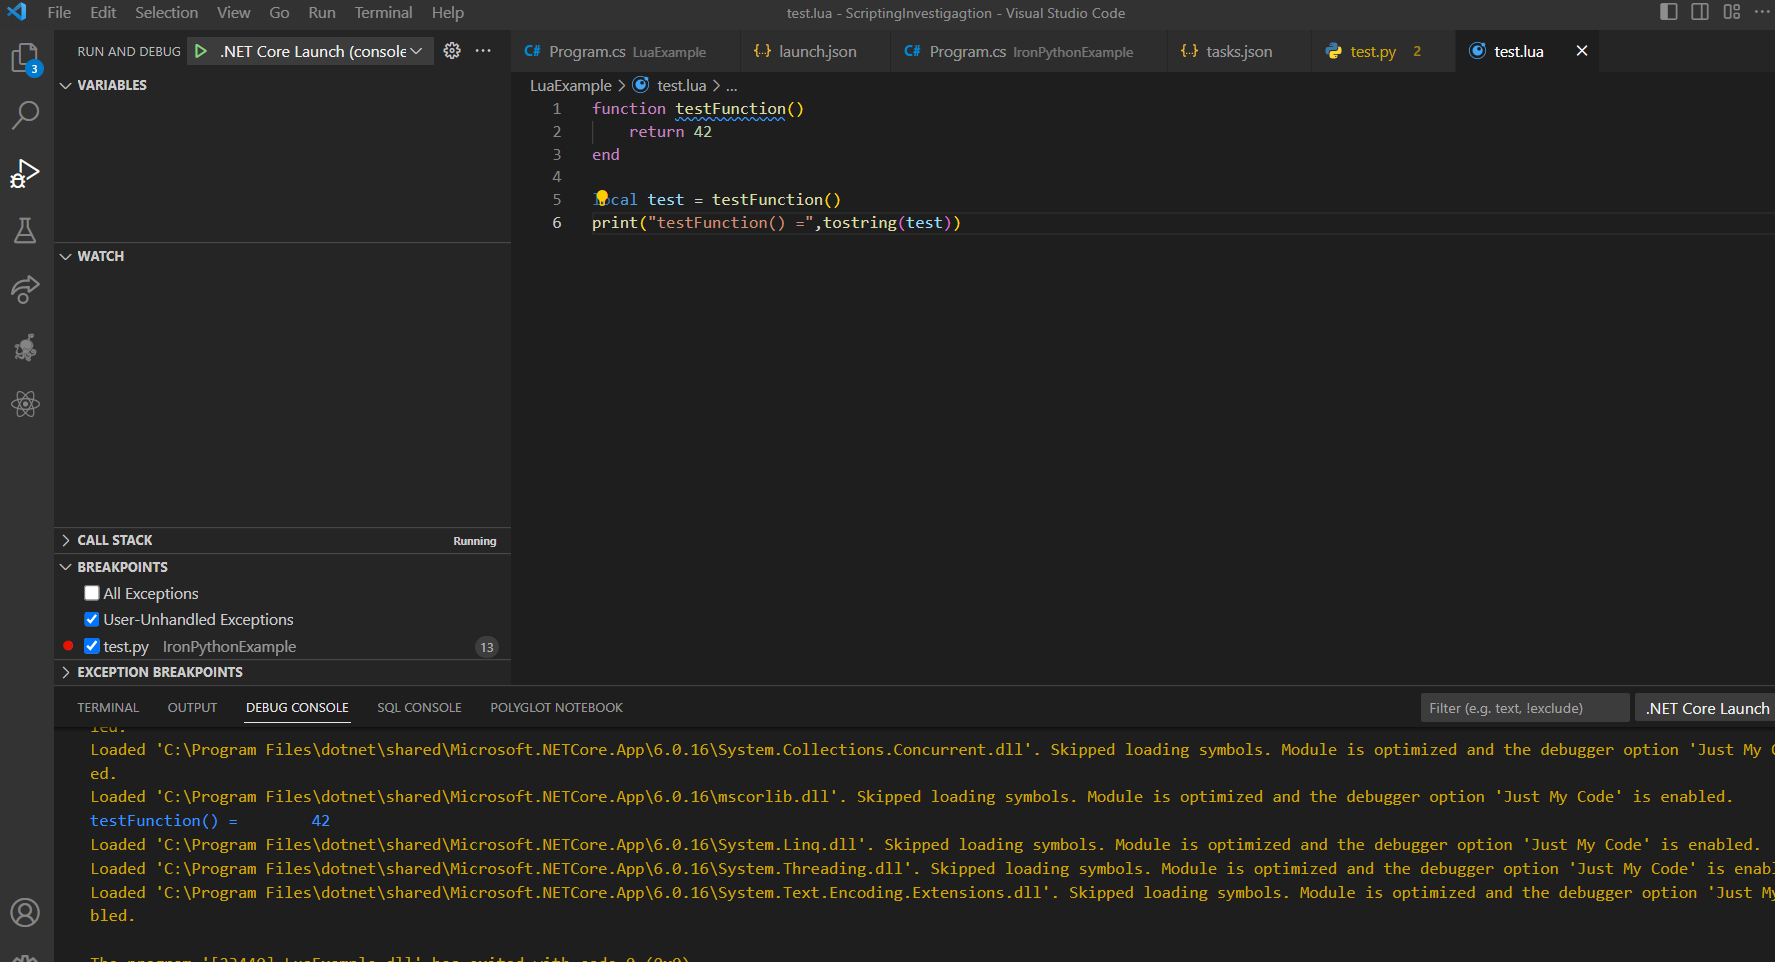
\includegraphics[scale=0.5]{pics/Lua-Konsolenausgabe.png}
        \caption{Lua-Konsolenausgabe}
        \label{fig:impl:KonsolenausgabeLua}
    \end{figure}

\newpage
    \item Die Beweise für das Debugging mit IronPython:
    \begin{figure}[H]
        \centering
        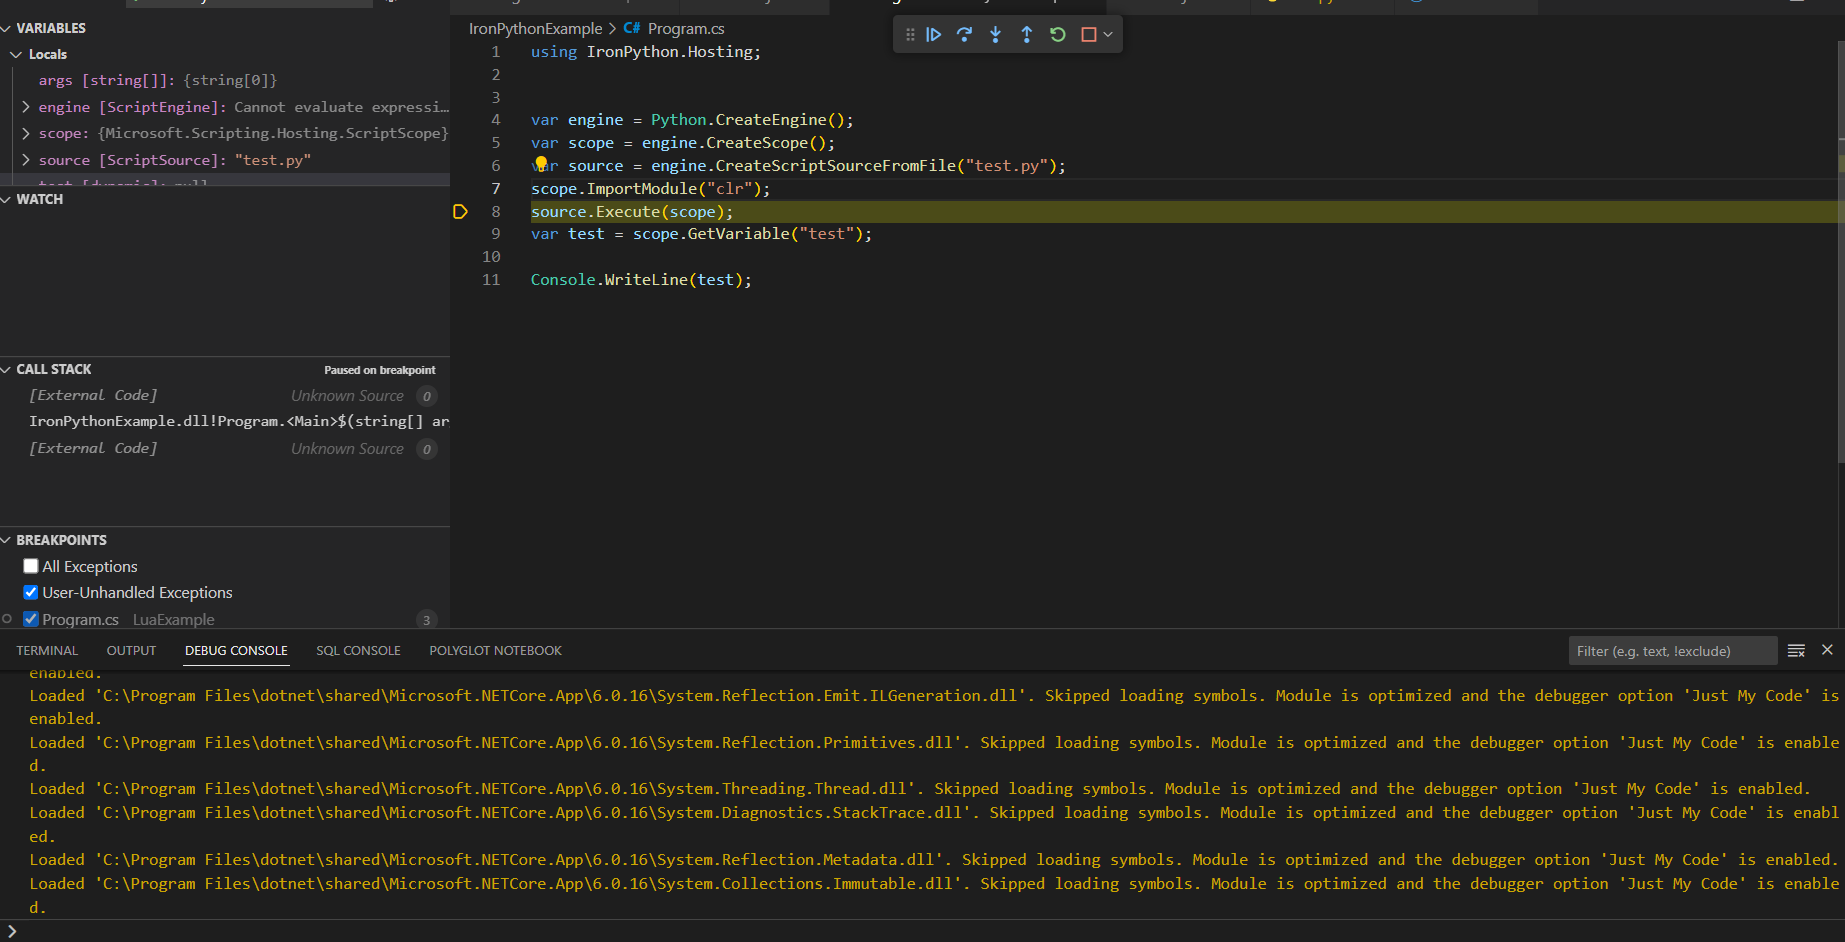
\includegraphics[scale=0.5]{pics/IronPythonVSCodeBreakpoint1.png}
        \caption{IronPython-VSCode-Breakpoint1}
        \label{fig:impl:IronPythonVSCodeBreakpoint1}
    \end{figure}

    \begin{figure}[H]
        \centering
        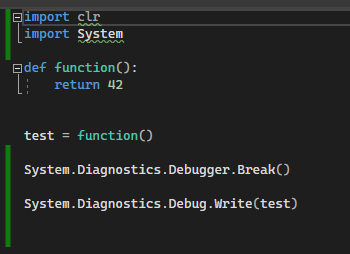
\includegraphics{pics/IronPythonVSBreakpoint2.png}
        \caption{IronPython-VSBreakpoint2}
        \label{fig:impl:IronPythonVSBreakpoint2}
    \end{figure}

    \begin{figure}[H]
        \centering
        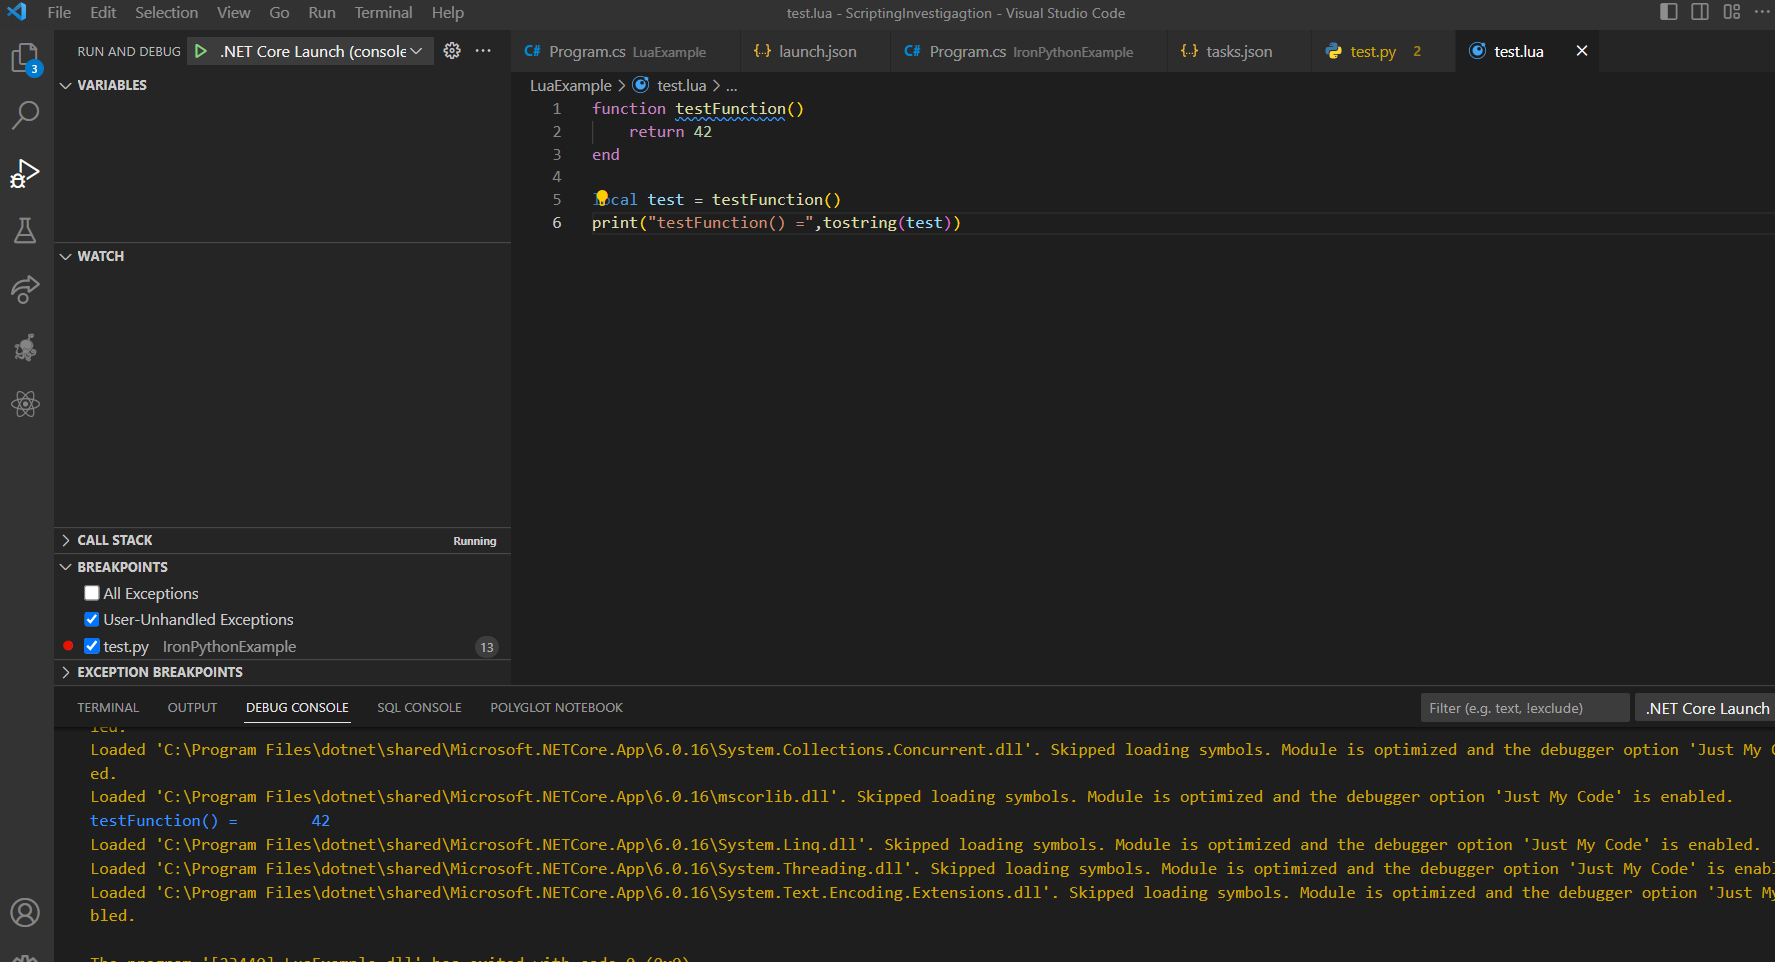
\includegraphics[scale=0.5]{pics/IronPythonKonsolenausgabe.png}
        \caption{IronPython-Konsolenausgabe}
        \label{fig:impl:IronPythonKonsolenausgabe}
    \end{figure}
\end{itemize}

\begin{spacing}{1}
\chapter{Anwendung (Praxisteil)}\label{chapter:tech}

\end{spacing}
\section{Verwendete Technologien}
\setauthor{Philipp Füreder}

\subsection*{ASP .NET Core}

Unsere Webanwendung wurde unter Verwendung der ASP.NET Core-Plattform entwickelt. 
ASP.NET Core ist ein vielseitiges, plattformübergreifendes und leistungsfähiges 
Open-Source-Framework, das zur Entwicklung moderner, internetfähigen Anwendungen geeignet ist. 
Die Ausführung findet in der .NET Core-Laufzeitumgebung statt.
ASP.NET Core bietet außerdem eine moderne und flexible Umgebung für die Entwicklung von Webanwendungen, 
die sowohl plattformübergreifend als auch hochgradig skalierbar sind.

Mit ASP.NET Core kann man:

\begin{itemize}

\item Webanwendungen und Webdienste, Internet-der-Dinge (IoT)-Anwendungen und 
mobile Backends entwickeln.
\item Auf verschiedene Betriebssysteme wie Windows, macOS und Linux arbeiten.
\item Anwendungen sowohl in der Cloud als auch auf lokalen Systemen bereitstellen.
\end{itemize}

Dieses Framework eröffnet somit eine breite Palette an Möglichkeiten für Entwickler, 
um moderne Anwendungen zu erstellen, die sich nahtlos mit dem Internet verbinden und 
sowohl in Cloud- als auch lokalen Umgebungen effizient betrieben werden können.
\newpage

\subsection*{Git}

Unsere Versionskontrolle haben wir mit Git gemacht. Git ist ein Versionskontrollsystem 
mit verteiltem Ansatz, das entworfen wurde, um sowohl kleine als auch äußerst 
umfangreiche Projekte auf schnelle und effiziente Weise zu verwalten.
Die Erlernbarkeit von Git gestaltet sich einfach, und seine geringe Systembelastung 
geht einher mit herausragender Performance. Es setzt sich von anderen Versionskontrollsystemen 
wie Subversion, CVS, Perforce und ClearCase ab, indem es Funktionen wie kosteneffiziente 
lokale „Branches“, bequeme Staging-Bereiche und vielfältige Arbeitsabläufe bietet.
Git erlaubt und begünstigt die Erstellung von mehreren unabhängigen lokalen Verzweigungen. 
Die Prozesse des Erstellens, Zusammenführens und Entfernens dieser Entwicklungsstränge 
nehmen lediglich Sekunden in Anspruch. \\

Git ist kostenfrei und Open-Source. Es wurde dazu entwickelt, Projekte aller 
Größenordnungen – von kleinen bis hin zu umfangreichen – schnell und effizient zu verwalten. 
Es zeichnet sich als Open-Source aus, da es die Anpassungsfähigkeit bietet, den Quellcode 
nach den individuellen Bedürfnissen der Nutzer/innen anzupassen. 
Mit seiner Open-Source-Natur ermöglicht Git mehreren Personen gleichzeitig an einem 
Projekt zu arbeiten und ermöglicht eine äußerst einfache und effiziente Zusammenarbeit. 
Aus diesem Grund wird Git als das herausragende Versionskontrollsystem betrachtet, 
das in der heutigen Zeit zur Verfügung steht.
\newpage

\subsection*{Docker}

Docker ist eine Plattform, welche Anwendungen gemeinsam mit ihren spezifischen Abhängigkeiten 
in Form von Containern bündelt. Dieser Ansatz gewährleistet, dass die Anwendung in 
jeder beliebigen Entwicklungsumgebung reibungslos funktioniert.
Jede einzelne Anwendung läuft in separaten Containern und verfügt über 
ihre eigenen Satz an Abhängigkeiten und Bibliotheken. Dies gewährleistet, dass jede 
Applikation in völliger Unabhängigkeit von anderen Anwendungen agiert und die Sicherheit gibt, 
dass sie Anwendungen erstellen können, welche sich nicht gegenseitig beeinträchtigen.
Wir haben in unserer Anwendung unser Frontend, Backend und die Datenbank über Docker laufen lassen.
Das heißt wir haben 3 Docker-Container benutzt. \\
 
Unter einem Container versteht man eine standardisierte Softwareeinheit, die sowohl den 
Programmcode als auch sämtliche damit verbundenen Abhängigkeiten zusammenfasst. 
Hierdurch wird sichergestellt, dass die Anwendung zuverlässig in unterschiedlichen 
Computerumgebungen ausgeführt werden kann. Ein Docker-Container-Image verkörpert eine 
autonome und ausführbare Softwareeinheit, welche sämtliche Komponenten für die Ausführung 
einer Applikation in sich trägt: den Code selbst, die Laufzeitumgebung, Systemwerkzeuge, 
Systembibliotheken und Konfigurationseinstellungen. \\

Container-Images verwandeln sich zur Laufzeit in eigenständige Container. 
Im Fall von Docker geschieht dies durch das Ausführen der Images auf der Docker Engine. 
Containerisierte Software steht sowohl für Linux- als auch für Windows-basierte Anwendungen 
zur Verfügung und gewährleistet eine gleichbleibende Ausführung, unabhängig von der genutzten 
Infrastruktur. Container schaffen eine Isolierung der Software von ihrer Umgebung und 
gewährleisten somit, dass die Anwendung konsistent arbeitet, selbst bei Unterschieden 
zwischen Entwicklungs- und Staging-Umgebungen.
\newpage
\subsection*{PostgreSQL}

Als Datenbanksystem haben wir uns für PostgreSQL entschieden, da wir bereits in anderen 
Projekten mit diesem gearbeitet haben. PostgreSQL ist Open-Source und verwendet die SQL-Sprache. 
Außerdem ist PostgreSQL auf allen gängigen Betriebssystemen kompatibel.
PostgreSQL läuft bei uns über Docker, somit haben wir nichts Zusätzliches dafür installieren müssen.
PostgreSQL ist sehr anpassbar, man kann beispielsweise eigene Datentypen 
definieren und individuelle Funktionen gestalten.\\

Datentypen in PostgreSQL:
\begin{itemize}
    \item Zahlen und Zeichen: Integer, Numeric, String, Boolean
    \item Strukturierte: Date/Time, Array, Range/Multirange
    \item Geometrisch: Point, Line, Circle, Polygon
    \item Anpassbare: Composite, Custom Types
\end{itemize}

Integrität der Daten:
\begin{itemize}
    \item UNIQUE, NOT NULL
    \item Primary Keys
    \item Foreign Keys
    \item Exclusion Constraints
    \item Explicit Locks, Advisory Locks
\end{itemize}


\newpage
\subsection*{BenchmarkDotNet (0.13.2)}

BenchmarkDotNet unterstützt Anwender/innen dabei, die Performance ihrer Methoden in 
Benchmark-Tests zu überprüfen. Ebenso ermöglicht es den Austausch von reproduzierbaren 
Messexperimenten. Diese Transformation gestaltet sich genauso unkompliziert wie die 
Erstellung von Unit-Tests. BenchmarkDotNet hilft dabei, übliche Fehler im Benchmarking-Prozess 
zu vermeiden und Nutzer zu informieren, sobald Unstimmigkeiten im Benchmark-Design oder den 
erfassten Messdaten auftreten. Die präsentierten Resultate erscheinen in einer 
nutzerfreundlichen Tabelle, die sämtliche relevanten Aspekte des Experiments herausstellt.\\
Anbei ein Beispiel von einem unserer BenchmarkDotNet-Tests:\\

\begin{lstlisting} [language={[Sharp]C},caption=BenchmarkDotNet,label=lst:impl:foo]
namespace C_SharpExample
{
    [MarkdownExporter,
        HtmlExporter,
        SimpleJob(RunStrategy.ColdStart, launchCount: 1, warmupCount: 5, targetCount: 5, id: "FastAndDirtyJob")]
    public class C_SharpTesting
    {
        [Benchmark]
        public void TestC_Sharp_Simple() => ReturnNumber();

        [Benchmark]
        public void TestC_Sharp_Sum() => MySum();

        #region C_SharpFunctions
        public static async void ReturnNumber()
        {
            var state = await CSharpScript.RunAsync("return 42;");
            Console.WriteLine(state.ReturnValue);
        }
        public static async void MySum()
        {
            var state = await CSharpScript.RunAsync("return 3 + 3;");
            Console.WriteLine(state.ReturnValue);
        }
        #endregion
    }
}
\end{lstlisting}

\newpage
\subsection*{Bogus}

Bogus haben wir in unserem Projekt für die Generierung von Fake Daten benutzt. 
Wir haben damit Schüler- und Lehrernamen erstellen lassen die wir in unserer Anwendung als 
Testdaten benutzt haben. Bogus funktioniert ausschließlich für 
.NET-Sprachen wie C\#, F\# oder VB.NET. \\

Es ist ganz unkompliziert zu verwenden. Wir haben in unserer Arbeit nur Namen generieren lassen, 
jedoch könnte man zu jedem Namen noch eine ganze Menge hinzufügen wie zum Beispiel 
Telefonnummern, E-Mail-Adressen, Wohnadressen oder auch die Herkunft.\\

Folgendes Codebeispiel zeigt die Generierung unserer Fake Daten für eine Schulklasse:\\

\begin{lstlisting} [language={[Sharp]C},caption=Bogus,label=lst:impl:foo]
            List<Student> firstStudents = new List<Student>();
                      
            #region Create Fake Students for each Schoolclass
            for (int i = 0; i < 10; i++)
            {
                var studentFaker = new Faker<Student>()
                    .RuleFor(x => x.Name, x => x.Person.FullName)
                    .Generate();
                firstStudents.Add(studentFaker);
            }
\end{lstlisting}

In der RuleFor() Methode kann man genau die Sachen angeben die man benötigt. 
In unserem Fall haben wir nur Vornamen und Nachnamen benötigt.


\newpage
\section{Aufbau}
\setauthor{Robert Freiseisen}

Um einen Überblick über die Beispielanwendung zu erhalten folgt nun ein Komponentendiagramm:

\begin{figure}[H]
    \centering
    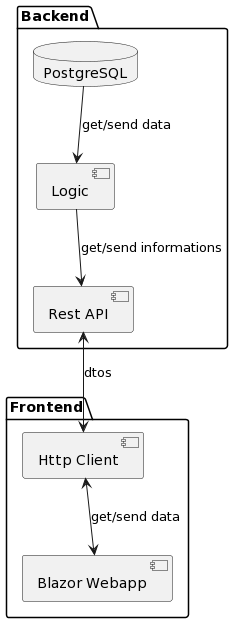
\includegraphics[scale=0.5]{pics/KomponentenDiagramm.png}
    \caption{Komponenten -- UML Diagramm}
    \label{fig:impl:KomponentenDiagramm}
\end{figure}

\newpage
Damit der Aufbau der .NET-Solution noch klarer wird ist nun die YAML-Datei dargestellt:

\lstinputlisting[style=yaml]{input-files/docker-compose.yml}

\newpage

Die verwendeten Entitäten und ihre Relationen im Backend sind in der folgenden Abbildung dargestellt.

\begin{figure}[H]
    \centering
    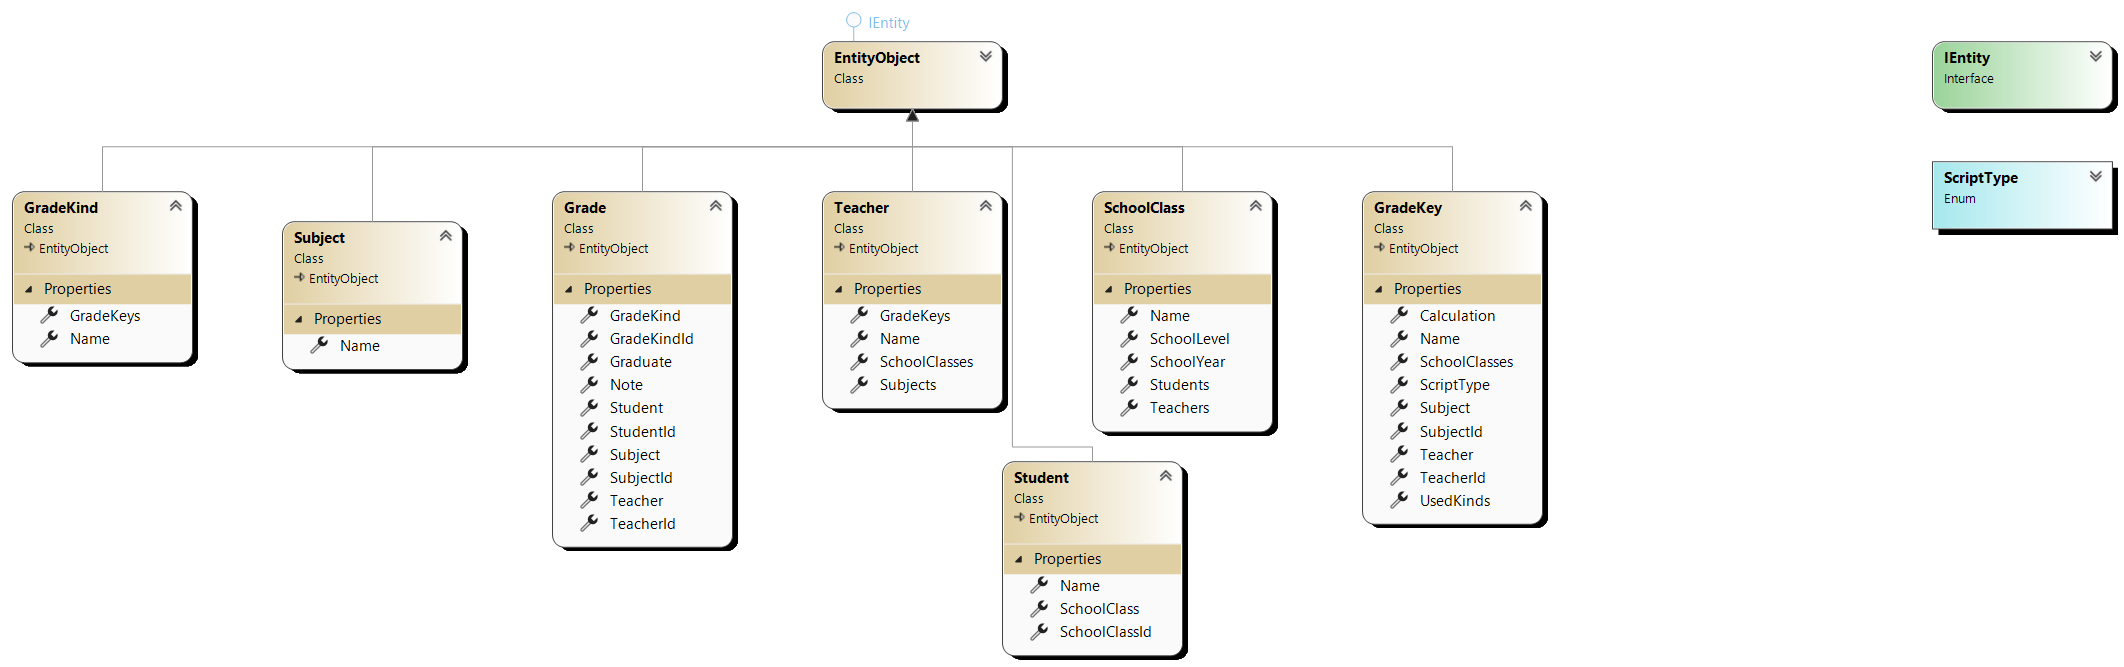
\includegraphics[scale=0.5]{pics/EntitiesClassDiagram.png}
    \caption{Entitäten -- UML Diagramm}
    \label{fig:impl:Entities}
\end{figure}

\newpage
Es gibt viele Möglichkeiten Skripte in eine Anwendung zu importieren.
Eine Möglichkeit ist die Skripte als Datei zu importieren.
Anstatt alle benötigten Daten direkt in den Code einzubetten oder sie manuell über die Befehlszeile einzugeben, 
können Entwickler eine oder mehrere Dateien als Input verwenden, die das Skript dann liest und verarbeitet.

\begin{figure}[H]
    \centering
    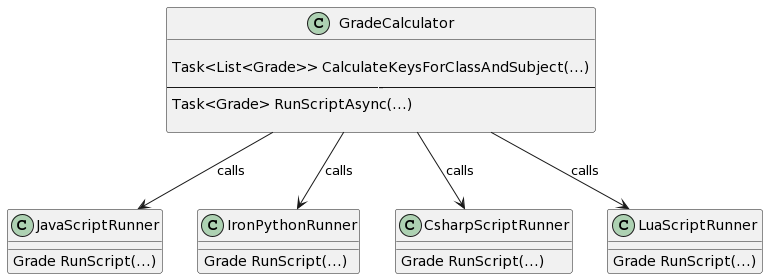
\includegraphics[scale=0.5]{pics/LogicClassDiagram.png}
    \caption{Logic Overview}
    \label{fig:impl:Logic}
\end{figure}


\newpage
Im folgenden Abschnitt  werden einige Code-Ausschnitte betrachtet, die zeigen, wie man solche Datei-Übergaben in den untersuchten Scriptsprachen realisieren kann. 

\begin{lstlisting}[language={[Sharp]C},caption=Code for Javascript,label=lst:impl:js]
    public class JavascriptRunner
    {
        public Grade RunScript(GradeKey key, List<Grade> grades)
        {
            var engine = new JintJsEngine();
            Grade result = new Grade();
            List<string>? logs = new List<string>();

            try
            {
                // Definiere eine Variable im JavaScript-Code, um die console.log-Ausgaben zu speichern
                engine.Execute("var consoleOutput = [];");

                // Definiere die console.log-Funktion im JavaScript-Code
                engine.Execute(@"
                                var console = {
                                    log: function() {
                                        consoleOutput.push(Array.from(arguments).join(' '));
                                    }
                                };
                            ");


                var gradeKindsList = JsonConvert.SerializeObject(key.UsedKinds);
                var gradesList = JsonConvert.SerializeObject(grades);

                engine.SetVariableValue("gradeKindsList", gradeKindsList);
                engine.SetVariableValue("gradesList", gradesList);

                if (key.Calculation != null)
                {
                    engine.Execute(key.Calculation);
                }

                //Die Ausgabe der console.log-Anweisungen als JSON-String
                string jsonOutput = engine.Evaluate<string>("JSON.stringify(consoleOutput)");

                // Konvertiere den JSON-String in eine Liste von strings
                if (jsonOutput != null)
                {
                    logs = JsonConvert.DeserializeObject<List<string>>(jsonOutput);

                    if (logs != null)
                    {
                        DisplayOutput(logs);   
                    }
                }

                // Get Return from Script
                var resultGrade = engine.GetVariableValue("result");

                result.Teacher = key.Teacher;
                result.Graduate = Convert.ToInt32(resultGrade);
            }
            catch (Exception)
            {
                result.Teacher = null;
                result.Graduate = 0;
            }
            return result;
        }

        private static void DisplayOutput(List<string> logs)
        {
            foreach (string output in logs)
            {
                Debug.WriteLine(output);
            }
        }
    }
\end{lstlisting}


\begin{lstlisting}[language={[Sharp]C},caption=Code for NLua,label=lst:impl:nlua]
    /// <summary>
    /// Runs lua-scripts
    /// </summary>
    public class LuaScriptRunner
    {
        private readonly Lua state;

        public LuaScriptRunner()
        {
            this.state = new Lua();
        }

        public Grade RunScript(GradeKey key, List<Grade> grades)
        {
            if (key.Calculation == string.Empty || key.UsedKinds == null || grades == null)
            {
                throw new NullReferenceException("Not enough information for Calculation");
            }

            var code = key.Calculation;

            var result = new Grade();
            try
            {
                state.DoString(code);
                state.LoadCLRPackage();
                state["grades"] = grades;
                state.DoString(@"graduate = calculate()");
                result.Teacher = key.Teacher;
                var gr = state["graduate"];
                if (gr != null) 
                {
                    result.Graduate = Convert.ToInt32(gr);
                }
            }
            catch (Exception)
            {
                throw;
            }

            return result;
        }
    }
\end{lstlisting}

\newpage

\begin{lstlisting}[language={[Sharp]C},caption=Code for CsharpScripting,label=lst:impl:csc]
    public class CsScriptRunner
    {
        public static Grade RunScript(GradeKey key, List<Grade> grades)
        {
            var result = new Grade();

            // StringWriter erstellen, um die Ausgabe des Skripts zu erfassen
            StringWriter sw = new StringWriter();

            // Console.Out umleiten
            TextWriter originalOut = Console.Out;
            Console.SetOut(sw);
            try
            {                
                dynamic script = CSScript.Evaluator
                    .ReferenceAssemblyOf(typeof(GradeKey))
                    .ReferenceAssemblyOf(typeof(Grade))
                    .CompileCode(key.Calculation)
                    .CreateObject("*");
                
                var res = script.Calculate(key, grades);
                result.Teacher = key.Teacher;              
                result.Graduate = Convert.ToInt32(res);

            }
            catch (Exception)
            {
                result.Teacher = null;
                result.Graduate = 0;
            }
            finally
            {
                // Output ausgeben
                Debug.WriteLine(sw);
            }

            return result;
        }
    }
\end{lstlisting}

\newpage
\section{Unit-Tests zur Überprüfung der Notenberechnung}
\setauthor{Philipp Füreder}

Eine der zentralen Komponenten unserer Beispielanwendung war die Implementierung von 
Skripten zur Notenberechnung in .NET-Anwendungen zur Laufzeit. Um die Zuverlässigkeit und 
Genauigkeit dieser Skripte sicherzustellen, haben wir einen Satz von Unit-Tests entwickelt 
und durchgeführt. Dieser Ansatz gewährleistet nicht nur die Integrität des Codes, 
sondern bietet auch eine robuste Basis für zukünftige Erweiterungen und Anpassungen.

\subsection*{Auswahl der Testfälle}
Die Testfälle wurden so ausgewählt, um ein breites Spektrum an Szenarien abzudecken, 
die in realen Anwendungen vorkommen könnten. Dazu gehören Standardfälle, Grenzfälle und 
auch potenzielle Fehlerzustände. Das hat uns ermöglicht, die Robustheit für unsere Test-Scripts 
umfassend zu überprüfen.

\subsection*{Ergebnisse der Unit-Tests}
Alle entwickelten Skripte zur Notenberechnung haben die Tests letztenendes erfolgreich bestanden. 
Dies gab uns ein hohes Maß an Vertrauen in die Funktionsfähigkeit und Zuverlässigkeit der 
implementierten Lösungen. Darüber hinaus haben die Tests dazu beigetragen, einige nicht 
offensichtliche Fehler und Unklarheiten im ursprünglichen Design zu identifizieren, 
die wir entsprechend beheben konnten.

\newpage
\subsection*{Testbeispiel}

In folgendem Testbeispiel haben wir ein C\#-Skript getestet:

\begin{lstlisting}[language={[Sharp]C},caption=Test for CsharpScripting,label=lst:impl:csc]
[TestMethod]
    public void CsScript_T02()
    {
        List<Grade> grades = new List<Grade>
        {
            new Grade { GradeKind = gradeKinds.Single(g => g.Name =="MAK") , Graduate = 1 },
            new Grade { GradeKind = gradeKinds.Single(g => g.Name =="MAK") , Graduate = 1 },
            new Grade { GradeKind = gradeKinds.Single(g => g.Name =="MAK") , Graduate = 1 },
            new Grade { GradeKind = gradeKinds.Single(g => g.Name =="MAK") , Graduate = 2 },
            new Grade { GradeKind = gradeKinds.Single(g => g.Name =="MAK") , Graduate = 1 },
            new Grade { GradeKind = gradeKinds.Single(g => g.Name == "TEST"), Graduate = 1},
            new Grade { GradeKind = gradeKinds.Single(g => g.Name == "TEST"), Graduate = 2},
            new Grade { GradeKind = gradeKinds.Single(g => g.Name == "TEST"), Graduate = 3},
            new Grade { GradeKind = gradeKinds.Single(g => g.Name == "TEST"), Graduate = 4},
            new Grade { GradeKind = gradeKinds.Single(g => g.Name == "TEST"), Graduate = 2},
            new Grade { GradeKind = gradeKinds.Single(g => g.Name == "HOMEWORK"), Graduate = 1},
            new Grade { GradeKind = gradeKinds.Single(g => g.Name == "HOMEWORK"), Graduate = 2},
            new Grade { GradeKind = gradeKinds.Single(g => g.Name == "HOMEWORK"), Graduate = 3},
            new Grade { GradeKind = gradeKinds.Single(g => g.Name == "HOMEWORK"), Graduate = 4},
            new Grade { GradeKind = gradeKinds.Single(g => g.Name == "HOMEWORK"), Graduate = 5},

        };

        var code = File.ReadAllText("test.cs");
        var key = new GradeKey { Name = "CsScriptTest", UsedKinds = gradeKinds, Calculation = code };

        var result = CsScriptRunner.RunScript(key, grades);

        Assert.AreEqual(2, result.Graduate, "Calculation is right");
\end{lstlisting}

Dabei beinhaltet die Liste "grades" Schulnoten von drei verschiedenen Typen:
\begin{itemize}
    \item MAK (Mitarbeitskontrolle)
    \item Test
    \item Homework
\end{itemize}


\newpage
\subsection*{Test-Skript}
Dieses Test-Skript haben wir geschrieben um die Funktionalitäten und Notenberechnungen zu testen.
Einfachheitshalber wird in diesem Skript jeder Notentyp äquivalent gerechnet.

\begin{lstlisting}[language={[Sharp]C},caption=CsharpScript-Testscript,label=lst:impl:csc]
int makCounter = 0;
int testCounter = 0;
int homeworkCounter = 0;

int mak = 0;
int test = 0;
int homework = 0;

foreach (var item in Grades)
{
    if (item.GradeKind.Name == "MAK")
    {
        mak += item.Graduate;
        makCounter++;
    }
    if (item.GradeKind.Name == "TEST")
    {
        test += item.Graduate;
        testCounter++;
    }
    if (item.GradeKind.Name == "HOMEWORK")
    {
        homework += item.Graduate;
        homeworkCounter++;
    }
}

return ((mak / makCounter) + (test / testCounter) + (homework / homeworkCounter)) / 3.0;
\end{lstlisting}

Das Skript unterscheidet zwar zwischen allen Notentypen, wertet jedoch alle gleich 
und berechnet den Durchschnitt.


\begin{spacing}{1}
\chapter{Technologien}\label{chapter:tech}
\end{spacing} 

\begin{spacing}{1}
\chapter{Umsetzung}\label{chapter:implementation}
\end{spacing}




\begin{spacing}{1}
\chapter{Zusammenfassung}
\end{spacing}
Aufzählungen:

\begin{compactitem}
    \item Itemize Level 1
    \begin{compactitem}
        \item Itemize Level 2
        \begin{compactitem}
            \item Itemize Level 3 (vermeiden)
        \end{compactitem}
    \end{compactitem}
\end{compactitem}

\begin{compactenum}
    \item Enumerate Level 1
    \begin{compactenum}
        \item Enumerate Level 2
        \begin{compactenum}
            \item Enumerate Level 3 (vermeiden)
        \end{compactenum}
    \end{compactenum}
\end{compactenum}

\begin{compactdesc}
    \item[Desc] Level 1
    \begin{compactdesc}
        \item[Desc] Level 2 (vermeiden)
        \begin{compactdesc}
            \item[Desc] Level 3 (vermeiden)
        \end{compactdesc}
    \end{compactdesc}
\end{compactdesc}

\newpage
\pagenumbering{Roman}
\setcounter{page}{\value{RPages}}
\newacronym{guid}{GUID}{Globally Unique Identifier}
\newacronym{jit}{JIT}{Just In Time Compiler}
\newacronym{nfc}{NFC}{Near Field Communication}
\newacronym{rfid}{RFID}{Radio Frequency Identification}

% Usage:
% \gls{label} lowercase in text
% \Gls{label} Uppercase in text
% \newacronym{label}{abbrev}{full}
% \newglossaryentry{label}{settings}



%\setlength{\glsdescwidth}{0.8\linewidth}
\glsnogroupskiptrue
\printglossary[title=Glossar,toctitle=Glossar] %,style=long]
\spacing{1}{
%\bibliographystyle{IEEEtran}
\bibliographystyle{ieeetrande}
\bibliography{bib}
}
\listoffigures
\listoftables
\lstlistoflistings
\appendix
\addchap{Anhang}
\input{./sections/appendix}
\end{document}